\chapter{Background}
% 10-20 pages
% This should form the bulk of the interim report. 
% You should consider that your objective here is to produce a near final version of the background section, as it will appear in your final report. 
% All of this material should be re-usable, so it is worth getting it right at this stage of the project.  
% The details of what to include can be found in the Project Report guidelines.

% - Perching Approaches
% - Reinforcement Learning
%   - Traditional
%     - FYP11 - Review Paper - maybe just discuss some findings
%     - Previous Work - done
%     - FYP8 - Human-Level Control through Deep Reinforcement Learning
%     - FYP12/23 - Autonomous Waypoint Navigation
%     - FYP13 - Noise Injection
%   - Apprentiship Reinformcent Learning 
%     - FYP7 - "An Application of Reinformcent Learning to Aerobatic Helicopter Flight (P. Abel 2007)" - done
%   - Demonstration
%     - FYP9 - DeepQ Learning from Demonstration - done
%     - FYP14 - Learning from Imperfect Demonstrations
%     - FYP-16 - Forgetful Experience Replay in Hierechical Reinforcement Learning from Expert Demonstrations.
%     - FYP17 - Mapless navigation for UAVs via Reinforcement Learning - done
%   - Transfer Learning
%     - FYP10 - Soft Actor-Critic with Inhibitory Networks for Retraining UAV Controllers Faster
%     - FYP18 - Inverse Reinforcement Learning
%   - Learned Skills
%     - FYP-15 - Demonstration Guided Reinforcement Learning with Learned Skills

% Previous Work - Fabian
The aim of this chapter is to provide an extensive review of perching techniques and automated trajectory generation, with a particular focus on methods that require minimum simulation interaction.
In order, we will cover various perching approaches, previous work on automated perching, reinforcement learning, experience replay, inverse reinforcement learning, learning from demonstrations and transfer learning.
\section{Perching Approaches}


There is currently huge interest in deploying UAVs in a variety of environments and conditions, this has motivated many innovative approaches to drone landing and perching.
Much of the existing body of research predominantly focuses on the mechanical mechanisms involved in enabling drones to perch.
For example work enabling drones to perch on uneven ground~\cite{perching-uneven-ground} or water surfaces~\cite{perching-water1,perching-water2}, with the assistance of a human pilot.

Some of the most notable approaches involve the utilisation of vacuum cups, allowing UAVs to attach securely to vertical surfaces such as walls~\cite{perching-vertical-surface}.
This method employs the force of a vacuum to attach the UAV to the surface, this allows for easy attachment and detachment through adjusting the pressure of the cup.
Magnetic mechanisms have also been explored~\cite{perching-magnets}.
However, their use is inherently limited to surfaces that are made of magnetic materials, which renders them less feasible for a forest environment unless magnetic surfaces are preinstalled in prticular locations.

\begin{figure}[ht]
  \centering
  \begin{subfigure}[b]{0.45\textwidth}
      \centering
      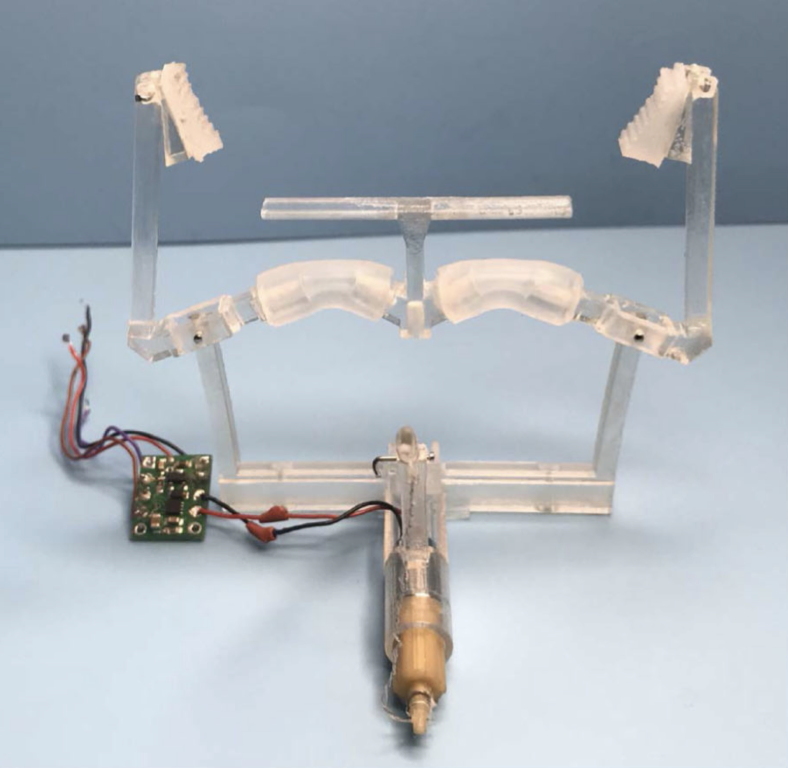
\includegraphics[width=\textwidth]{background/perching-gripper1.png}
      \caption{Gripper activated by force pushing against a branch taken from~\cite{perching-gripper1}}
      \label{fig:perching-gripper1}
  \end{subfigure}
  \hfill
  \begin{subfigure}[b]{0.45\textwidth}
      \centering
      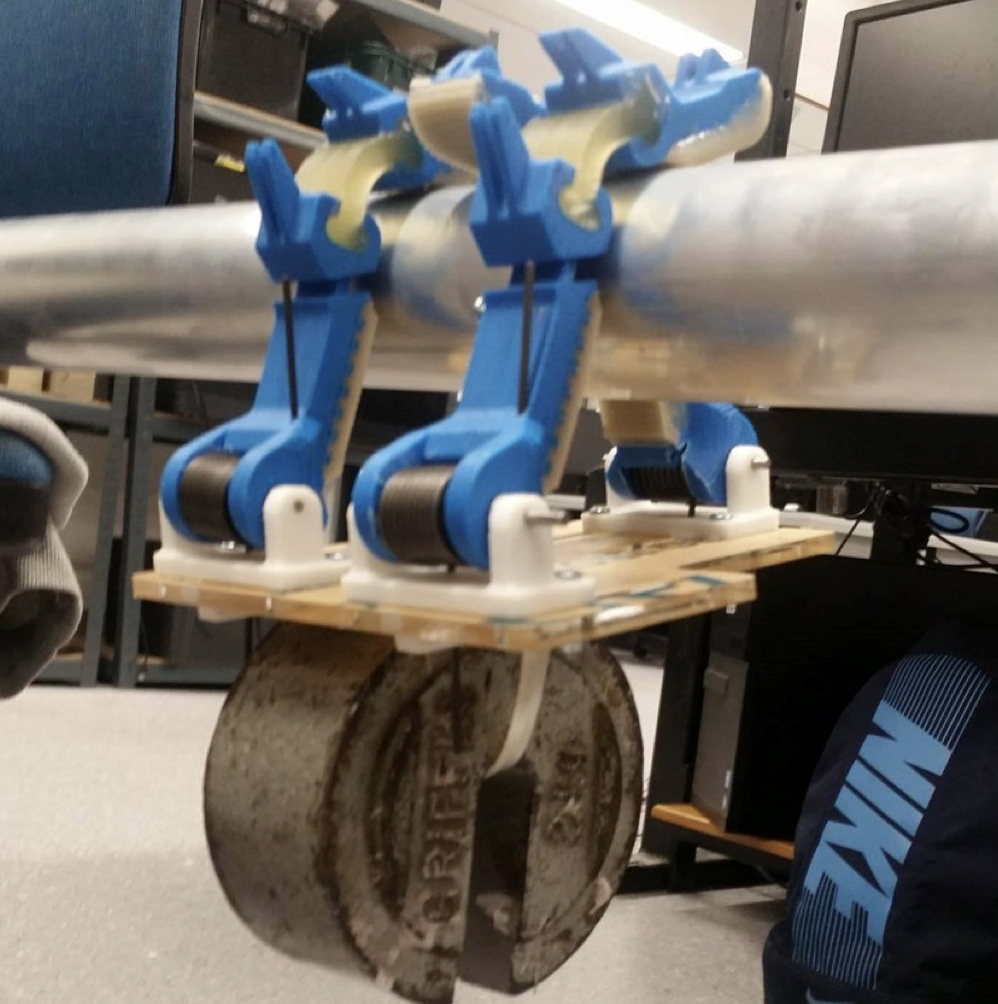
\includegraphics[width=\textwidth]{background/perching-gripper2.png}
      \caption{Gripper utilising a three-fingered robotic arm taken from~\cite{perching-gripper2}}
      \label{fig:perching-gripper2}
  \end{subfigure}
  \caption{Perching Mechanisms for use in a forest environment}
  \label{fig:perching-grippers}
\end{figure}

The focus of this project is the application of drones within forest environments, particularly for environmental sensing tasks. 
In line with this objective, numerous studies have developed mechanical mechanisms that would be suitable for attachment to a tree branch. 
Again the majority of the existing research in the area focuses on the mechanical mechanism with which attachment is achieved. 
Examples include the work by H. Zhang et al~\cite{perching-gripper1}, which discusses a gripper mechanism activated upon pushing against a branch, as depicted in Figure~\ref{fig:perching-gripper1}. 
Additionally, the research by A. McLaren et al~\cite{perching-gripper2} presents a sophisticated approach involving a three-fingered robotic hand, as illustrated in Figure~\ref{fig:perching-gripper2}.
This hand wraps around a tree branch-like structure to keep the drone perched.


\begin{figure}[htbp]
  \centering
  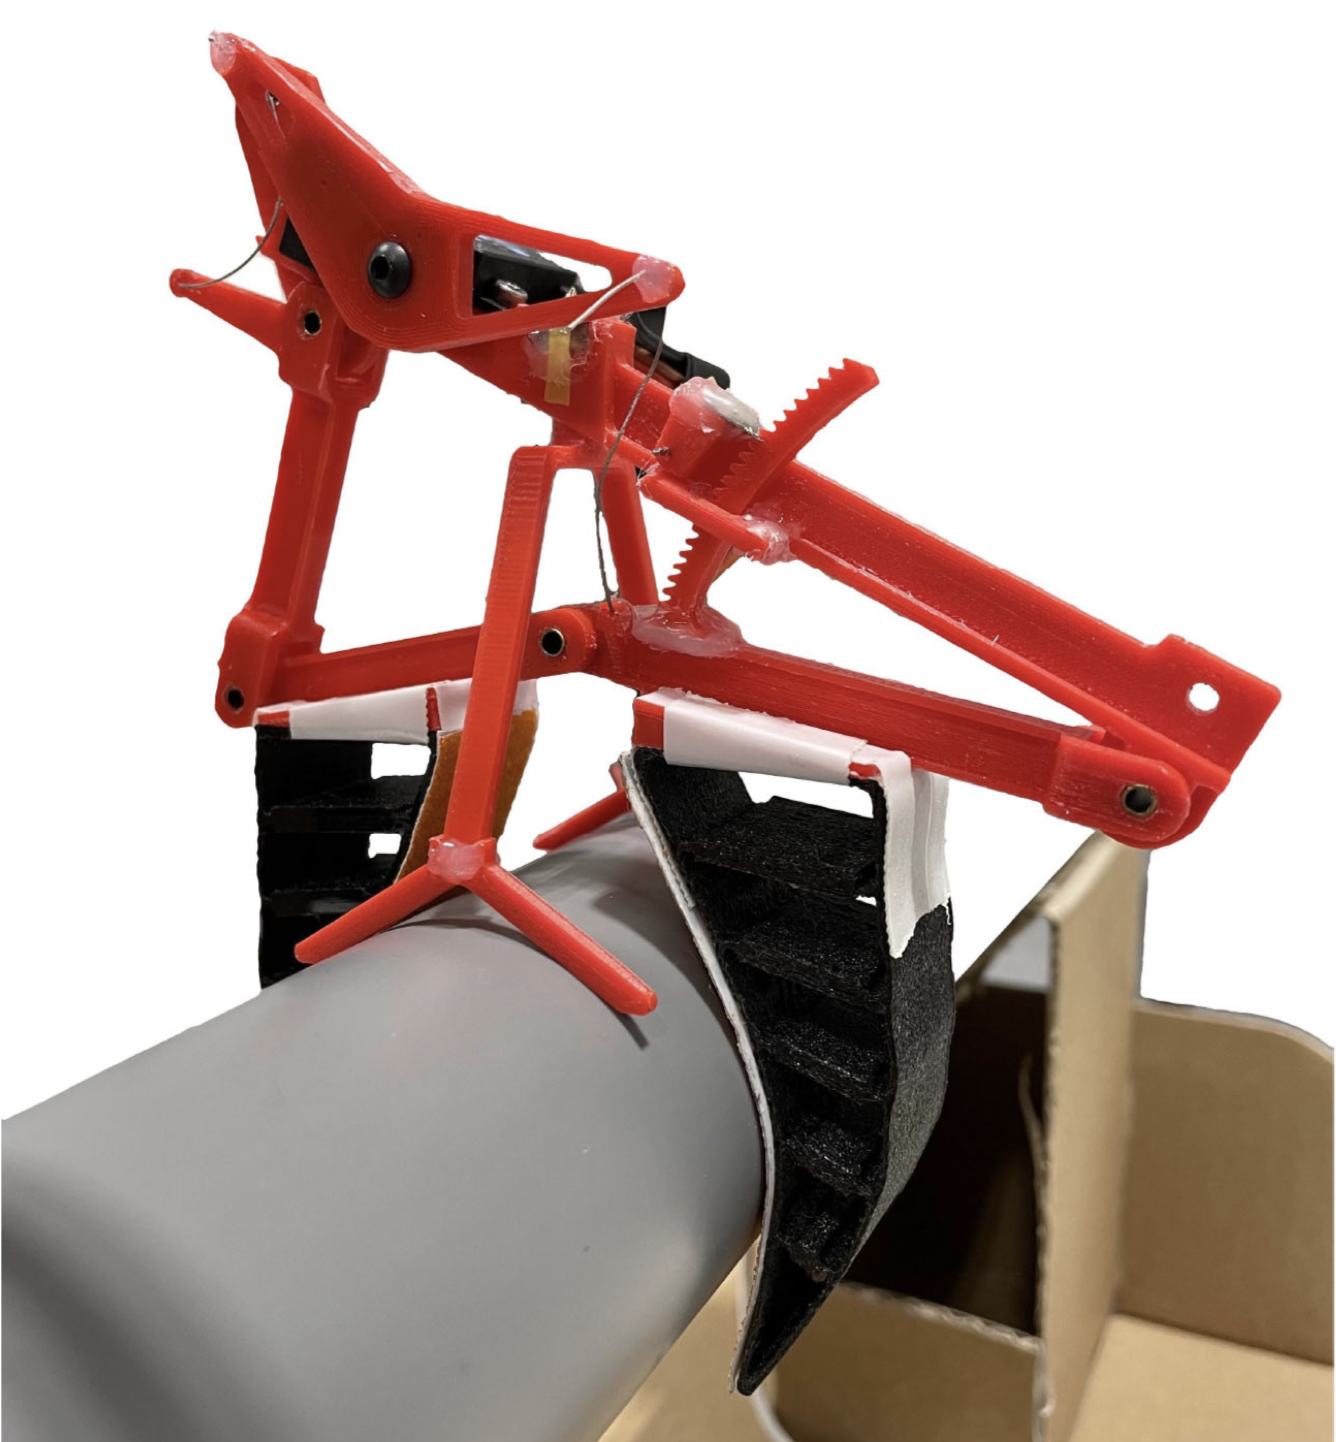
\includegraphics[width=0.5\textwidth]{background/perching-tum.png}
  \caption{Bird-inspired perching on a branch taken from~\cite{perching-tum-bird}}
\label{fig:perching-tum-bird}
\end{figure}

Bioinspired perching mechanisms have also been proposed for UAVs~\cite{perching-tum-bird} utilising bird-feet style gripers to attach to a branch-like structure.
This mechanism has the ability to exert a significant gripping force while consuming minimal power.
To date, a prototype has been successfully tested, demonstrating its ability to perch onto a variety of branch-like objects under the control of a human pilot.

As discussed, much of the existing literature predominantly concentrates on the mechanical attachment process for the UAV.
This project will instead focus towards a more flight-oriented approach.
We will utilise a simple bioinspired tethered drone, as depicted in Figure~\ref{fig:background-tethered-drone}, and aim to automate the perching process.
This UAV design incorporates a pendulum mechanism situated beneath the drone body, the pendulum is able to move freely under the drone.
This mechanism is extremely straightforward from a mechanical perspective, it does not require any specialised hardware and can easily be retrofitted onto an existing UAV.
Furthermore, unlike many other mechanical mechanisms, the diameter of the branch is not crucial, any branch that can hold the weight would be suitable.

\begin{figure}[H]
  \centering
  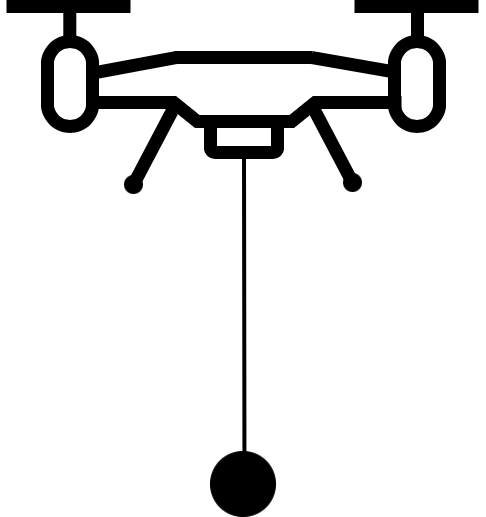
\includegraphics[width=0.33\textwidth]{introduction/TetheredDrone.drawio.png}
  \caption{Tethered Drone: A UAV with a tether attached to a small weight}
\label{fig:background-tethered-drone}
\end{figure}

The perching manoeuvre involves the drone wrapping its tether around a branch and slowly disarming to suspend itself beneath the branch. 
This state of suspension requires no energy to maintain. 
This is an extremely energy-efficient solution for a UAV and enables  the long-term monitoring of an environment. 
The detachment process involves the drone unravelling the tether from the branch before resuming flight. 
Previous work in this area has indicated the feasibility of executing the initial phase of this manoeuvre, as further discussed in Section~\ref{sec:background-prev-work}, this project aims to refine and complete the process. 
It aims to leverage innovative techniques to successfully execute the entire manoeuvre, thereby contributing to the advancement of UAV perching technology in real-world applications, in particular for dense forest environments.

\section{Previous Work}
\label{sec:background-prev-work}

% Previous Work

Previous work has explored the use of Reinforcement Learning in automatically generating trajectories for drone perching~\cite{learnedTetheredPerchingFabian}.
In this approach, a Soft Actor Critic algorithm was employed to develop a series of energy-optimised trajectories.
The trajectory was divided into three separate stages.
The initial approach and contact phases used trajectories formulated using analytical solutions.
The Reinforcement Learning aspect was specifically applied for the more complex manoeuvre of flipping the drone beneath the branch.

\todo{diagram for this manoeuvre}
\begin{figure}[htbp]
  \centering
  
\includegraphics[width=0.33\textwidth]{frog.png}
  \caption{TODO}
\label{fig:previous-work-manuever-diagram}
\end{figure}

\todo{diagram for this manoeuvre}
\begin{figure}[htbp]
  \centering
  
\includegraphics[width=0.33\textwidth]{frog.png}
  \caption{TODO}
\label{fig:previous-work-rolling}
\end{figure}

The disarming manuever is shown in more detail in Figure~\ref{fig:previous-work-rolling}.
For this manuever, a Markov Decision Process was defined using observations $o_{t} \in O$ where $o_{t}$ denotes the drone's relative position and $a_{t}$ determines its roll rate.
A single demonstration using a constant roll rate was utilised as a baseline.
Two components of a reward function were used during training.
In the initial training stages, the algorithm prioritised conforming to the provided baseline.
As training progresses, reward shaping was used to shift the focus of the reward function, increasingly favouring a faster, more energy-efficient trajectory.
This allows for some exploration of the parameter space.

\[
R_{1}(s_{t}, a_{t}) = 
\begin{cases} 
I(s_{t}, a_{t}) & \text{for } t \leq t_{I} \\
I(s_{t}, a_{t}) M(t) & \text{else} 
\end{cases}
\]

\[I(s_{t}, a_{t}) = 3 \times 10 ^ 5 \times (0.1 - \min(|s_{\alpha} - s'_{\alpha}|, 0.1)) ^ 4\]
\[M(t) = \frac{t_{\max} - t}{t_{\max} - t_{I}}\]

\[
R_{2}(s_{t}, a_{t}) =
\begin{cases}
  R_{L} + \frac{\Delta X_{target} - 0.005}{l_{r}} \times 50 & \text{for } \frac{d_{target}}{d_{drone}} > 1 \\
  R_{L} + \frac{\Delta X_{branch}}{d_{drone}} \times 100 & \text{else}
\end{cases}
\]

\todo{rephrase this section}
where $s_{\alpha}$ and $s_{\alpha}$ are the roll angel of the current and the baseline state; 
$t_{\max}$ is the maximum time of the simulation; 
$t_{I}$ is the time when the final point should be reacted.
where RL is the reward from the last step dtarget is the distance to the target position; 
ddrone is the size of the drone; 
$\delta$Xtarget and $\delta$Xbranch is the change in the distance made to the final position and to the branch, and lr is the length of the rope.

However, this method constrains the range of possible solutions.
Favouring approaches that resemble the baseline, could prevent the system from learning novel, potentially more efficient strategies.
Since just roll rate was explored, this limits the range of solutions which reduces the computational complexity but may not fully explore paths.
Additionally one of the main challenges in the previous work was simulation.
Accurately modelling the dynamics between the tether and the drone presented significant challenges.
Performing training in a real-world setting would be exceptionally difficult, given the extensive number of trials required and the risk of errors causing physical damage to the drone.

This, therefore, presents a need to devise a system capable of efficiently learning from a very limited number of experiments while ensuring the safety of the drone. \\\\

\section{Reinforcement Learning}
% Intro
Reinforcement learning involves an agent that interacts with an environment to gain knowledge and receive feedback in the form of rewards~\cite{rlIntroSuttonBarlo}.
The agent explores the environment, discovers which actions yield the most reward, and then refines its strategy to produce an optimal policy.
States are a mathematic representation of the environment, and must contain all information required to compute the optimal policy.
Within the particular task of drone perching, this is likely to include coordinate positions along 3 dimesnions and angles along all axes.
The actions here represent what the drone will execute to solve the problem which for this problem represents the velocities in the trajectory.

\todo{do this diagram and finish the text above}
\begin{figure}[htbp]
  \centering
  
\includegraphics[width=0.33\textwidth]{frog.png}
  \caption{TODO}
\label{fig:rl-intro-drone}
\end{figure}

% FYP11 - Review Paper - maybe just discuss some findings
The problem of trajectory generation for drone perching has a large overlap with UAV navigation.
Therefore when investigating work on reinforcement learning this was a particular area that was focussed on since the objective is largely the same.
In 2022 a review paper~\cite{aerialNavReview} on UAV navigation using RL identified 159 papers that use RL to solve UAV navigation challenges.
Within path planning the review described papers based on both mapless and map-based navigation.
A map-based navigation approach uses an internal representation of the area, largely including terrain or obstacles.
Within drone perching this would likely relate to s \todo{finish this}

However one of the major limitations of traditional reinforcement learning in this context is the high number of episodes required to train.
For navigation tasks, this can be simulated reasonably well, however, as discussed in Section~\ref{sec:background-prev-work}, this is more difficult. \\\\

% FYP8 Human-Level Control through Deep Reinforcement Learning
The development of Deep Q-Networks utilising neural networks combined with reinforcement learning has proved extremely successful in the Atari Games, a popular benchmark in RL.
Human-level control was achieved in the Atari Gameset using a deep Q-network (DQN)~\cite{humanLevelControlDQN}.
This was primarily due to the innovative approximation of the Q-value function using a neural network.
Another one of the major innovations was the use of experience replay.
This involves storing experiences in a replay buffer and randomly sampling mini-batches.
Since deep neural networks require a large amount of data to train, experience replay significantly enhances the efficiency of data by reusing
This approach in turn drastically reduces the number of episodes required for effective training.
Building on this, some techniques have gone beyond random sampling to incorporate strategies such as prioritising experiences that lead to the most substantial changes in network weight.
This is discussed further in Section~\ref{sec:background-experience-replay}.

Another key component of the success was the use of frame-skipping and stacking techniques.
The system stacks 4 frames on top of each other for each pass, this potentially provides the network some insights into the changes between frames.
Additionally frame skipping was used, with a 10Hz sampling rate applied to the game.
This reduced the amount of data and therefore the number of steps required, emulating what a human would be capable of.

The real benefit of this approach is its ability to reduce the overall simulation time.
For the Atari Games, computing an action was significantly more computationally expensive than performing a simulation step.
However, in real-world tasks, the situation might be reversed, with the actual execution of the tasks being more time-consuming than simple decision-making.
Increasing the sampling rate for a drone application will increase the amount of data collected, which could lead to more being learned from each run.
It will therefore be interesting to examine this particular propery in a drone environment. \\\\

%     - FYP12/23 - Autonomous Waypoint Navigation

In the area of autonomous waypoint navigation, various methods have been explored and implemented.
One of the primary challenges is operating in a continuous environment, which adds complexity to the training process.
A common strategy involves discretising the environment, enhancing the performance by simplifying the state space.
However this sacrifices flexibility for performance.
The nature of the continuous environment is often lost and navigation becomes inherently more intricate.
A drone moving in a discretised environment would transition from point to point, resulting in neither a smooth nor efficient path.
This leads to trajectories that are unstable and inefficient.
To deal with this, a substantial increase in the number of states is required.
However, this loses much of the previously gained benerfit and this negatively impacts performance, particularly in a three-dimensional Euclidean space where drones operate with six degrees of freedom.

An interesting approach to deal with these issues was proposed to use waypoints and Bezier curves to define a trajectory~\cite{fyp12-waypoint-navigation}.
This approach splits the system into two distinct parts as shown in Figure~\ref{fig:fyp12-waypoint-nav-framework}.
The high-level component focuses on choosing waypoints that minimise thrust cost, thereby reducing energy usage.
The lower-level component creates smooth trajectories through these waypoints and provides a cost evaluation.
The overall goal of the system is to produce seamless trajectories that avoid obstacles within known 3D environments.
This goal significantly resembles the drone perching task, making it an interesting paper to examine.

\todo{do this diagram}
\begin{figure}[htbp]
  \centering
  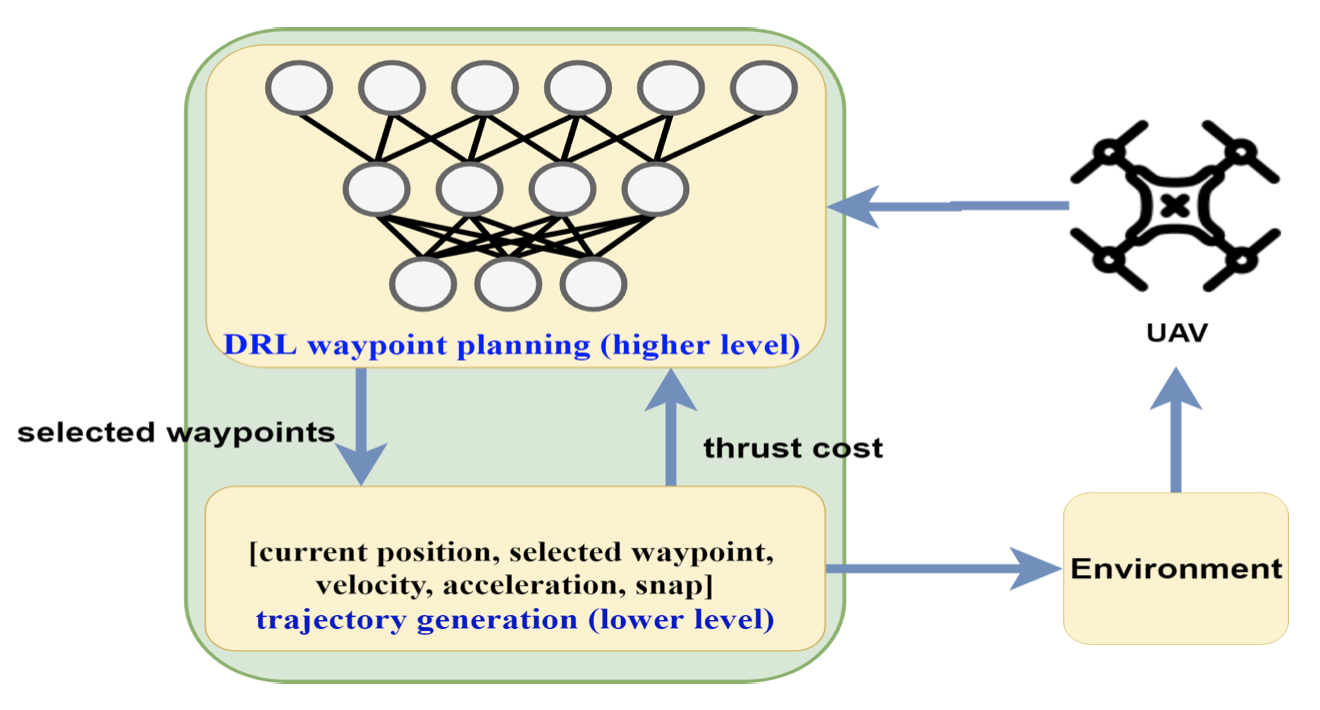
\includegraphics[width=0.5\textwidth]{background/fyp12-waypoint-nav-framework.png}
  \caption{Waypoint Navigation Framework}
\label{fig:fyp12-waypoint-nav-framework}
\end{figure}

At the higher level, the system utilises a Deep Q-Network (DQN).
The 3D environment is discretised into an N x N x N grid, where actions are defined as potential waypoints in a 3 x 3 x 3 grid surrounding the current position.
This gives 26 potential actions for each state.
Convolutional Neural Networks (CNNs) are used to process the 3D input state (the known 3D environment) with a fully-connected output layer, with 26 neurons, each corresponding to one of the possible actions.

The reward is defined as the weighted sum of two components:
\[R(s, a) = \alpha R_{p} + \beta R_{c}\]

where $R_{p}$ is the position reward:
\[
R_{p}(s, a) = 
\begin{cases} 
10 & \text{reach the target position} \\
-10 & \text{collide with obstacle} \\
0 & \text{otherwise}
\end{cases}
\]

and $R_{c}$ represents the control reward, defined as the negative L1 norm of the thurst cost, provided by the lower level system.
This balances the reward between reaching targets, avoiding obstacles and minimising cost.
The lower-level system follows a more traditional control-based algorithm~\cite{fyp12-waypoint-nav2}.

This two-part system was a novel approach that significantly reduces the number of states in a discretised environment while still achieving a smooth, minimised trajectory.
It simplifies the reinforcement learning system to focus on the optimal positions rather than explicitly learning flight control.
However since this model is focused on obstacle avoidance and navigation, the state is simply made up of the translational coordinates.
For tasks such as perching, incorporating all 6 dimensions, including rotational ones, is likely to complicate computation further.
In previous work, occasionally the weight on the drone collided with either the string or the drone itself.
Treating the weight as an obstacle that could collide with itself could be an interesting approach to potentially reduce the chances of this happening.
However this would require modelling the position of the ehter which could potentially further complicate the environment, and make defining a reward function even more complicated to the point where it would be very challenging to manually define. \\\\

%     - FYP13 - Noise Injection
Noise Injection can be utilised within Deep Reinforcement Learning to mitigate the risk of overfitting and to foster the exploratory behaviour of the agent.
Specifically, the injection of Gaussian Noise has been investigated within the domain of UAV navigation~\cite{fyp13-noise-injection}, offering a promising approach to enhance the robustness and generalisation capabilities of the learning process.
This technique can be employed when the agent is required to make decisions from partial or noisy inputs like those from real-world experiments.
This system makes use of a Double Duelling Deep Q Network (D3QN) consisting of a CNN and a double duelling network as shown in Figure~\ref{fig:fyp13-d3qn-noise}.
This produces three possible discreet actions; move forward, yaw left or yaw right.
Gaussian Noise layers were introduced after the CNN and after the duelling neural networks.

\begin{figure}[htbp]
  \centering
  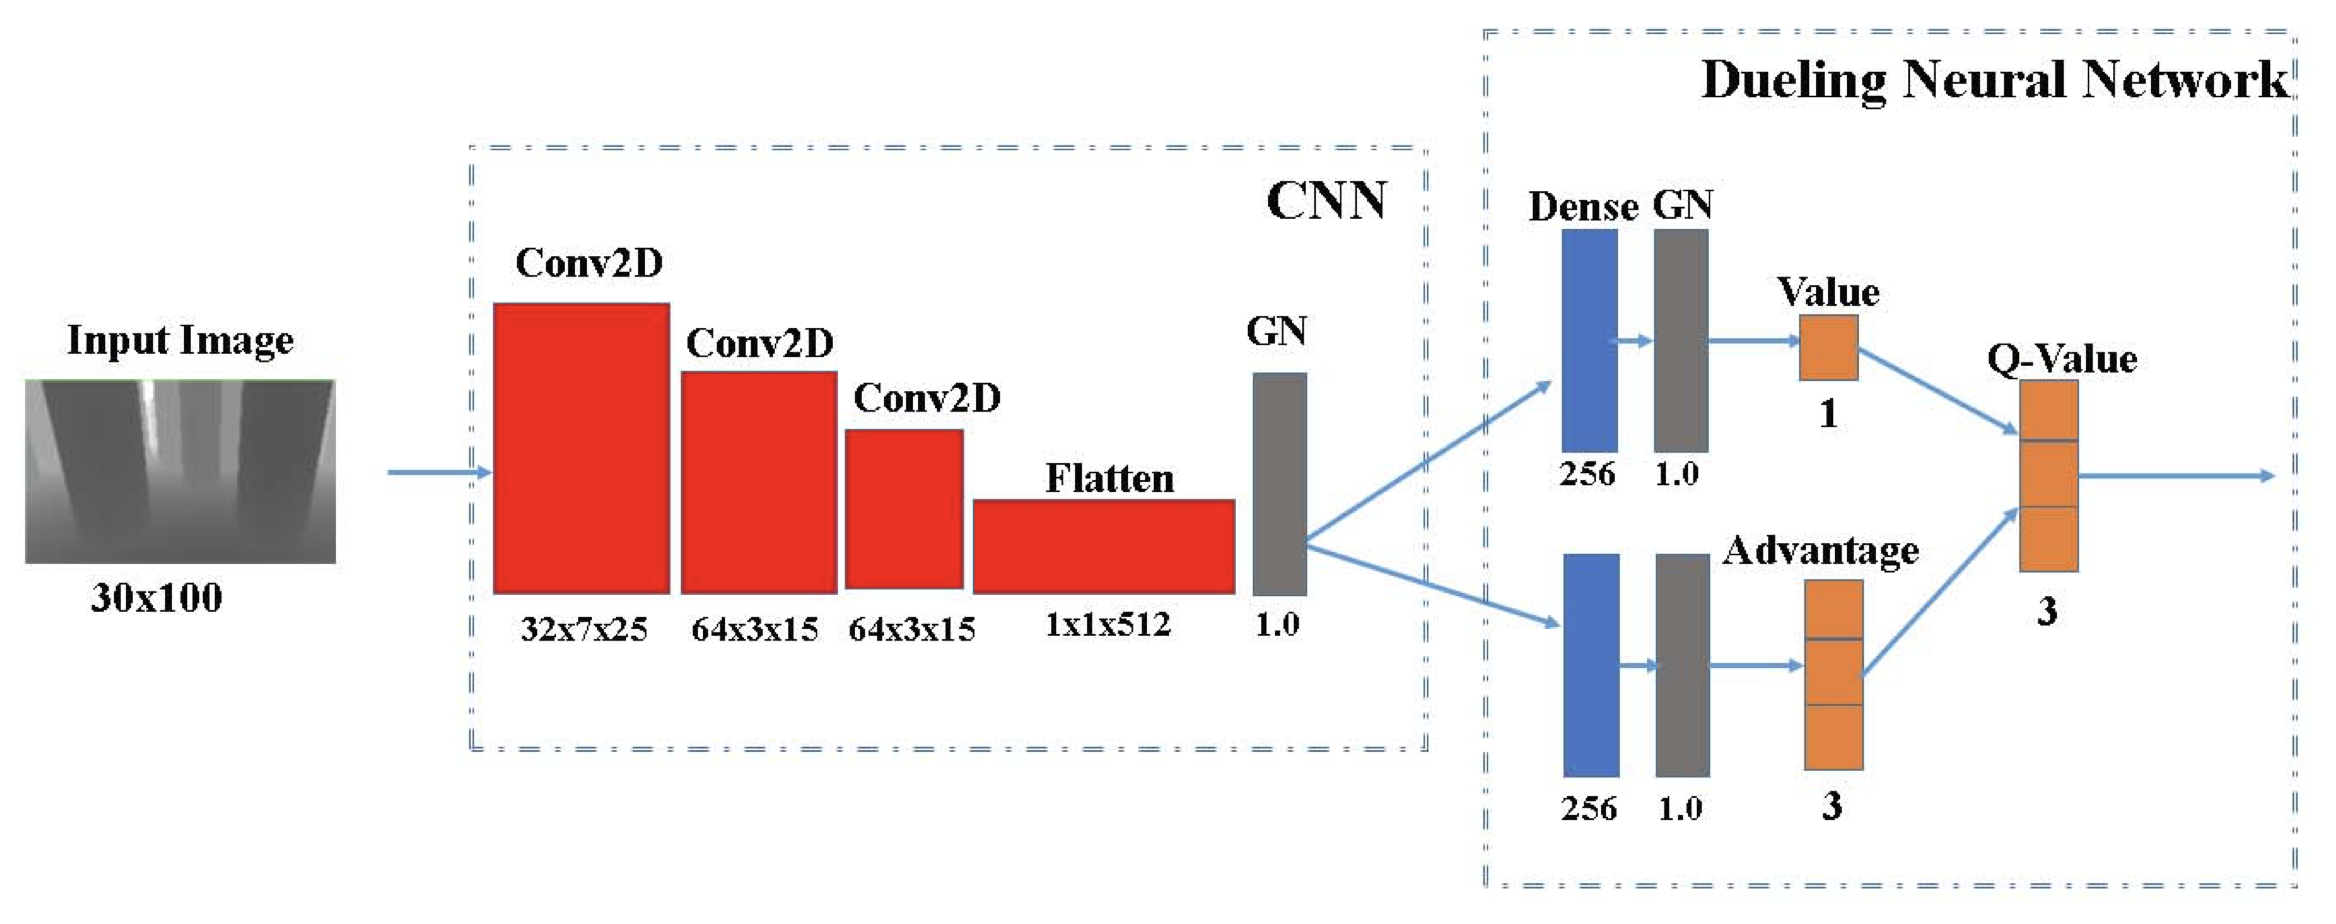
\includegraphics[width=0.5\textwidth]{background/fyp13-noise-injection.png}
  \caption{Double Duelling Deep Q Network with Gaussian Noise Injection}
\label{fig:fyp13-d3qn-noise}
\end{figure}

This architecture was then benchmarked against the standard D3QN in a path-planning scenrio that required obstacle avoidance.
The performance of the models over episodes is illustrated in Figure~\ref{fig:fyp13-results}.
The results indicate that while both algorithms converge to comparable Q values, the D3QN model with Gaussian Noise has a higher stability during the training phase.
Although these effects need further investigation within the specific environmental context, this approach is a potential practical tool to avert overfitting. 
This is particularly relevant when employing demonstration data, where the model's ability to generalise beyond the training samples is crucial. 
The introduction of Gaussian Noise as a form of regularisation in D3QN presents an innovative method to improve the robustness and reliability of an agent.

\begin{figure}[H]
  \centering
  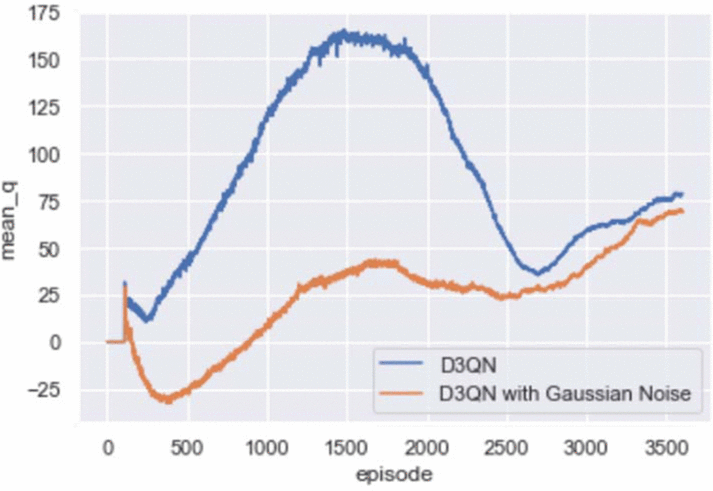
\includegraphics[width=0.5\textwidth]{background/fyp13-noise-results.png}
  \caption{Mean Q values of D3QN and D3QN with GN Injection}
\label{fig:fyp13-results}
\end{figure}

\section{Experience Replay}
\label{sec:background-experience-replay}

%     - FYP-16 - Forgetful Experience Replay in Hierechical Reinforcement Learning from Expert Demonstrations.

Experience Replay is an essential technique in Reinforcement Learning, significantly reducing the required number of episodes and, therefore, the number of demonstrations.
Adjusting the experience replay mechanism is critical for dealing with suboptimal or low-quality demonstration data.
Traditional RL methods typically replay samples at the same frequency as they were initially observed.
However, this approach may result in the loss of crucial samples, hindering the learning process.

A notable approach is the introduction of Prioritised Experience Replay~\cite{fyp-16-prioritised-experience-replay}, a methodology designed to select the best sampling of episodes. 
The core objective of Prioritised Experience Replay is to sample episodes that lead to more significant learning improvements for the agent. 
This corresponds to those episodes where the expected learning progress is maximized. 
A reasonable approximation for this metric is the magnitude of a transition's Temporal Difference (TD) error, $\delta$. 
This error is then used to form a prioritized sampling queue.

However, since the values associated with each experience are only updated when an experience is replayed, a purely greedy sampling approach will overlook episodes that initially have low scores.
To counter this limitation, a stochastic sampling method was introduced.

The probability of a transition being sampled is given by:

\[ P(i) = \frac{p_{i}^{\alpha}}{\sum_{k} p_{k}^{\alpha}} \]
where: $p_{i} = |\delta_{i}| + \epsilon$ and $\epsilon$ is a small positive constant that ensures every transition has a nonzero probability of being sampled.
While Prioritised Sampling is beneficial, it introduces some bias into the learning process, meaning that corrective measures are necessary. 
The importance sampling weight $w_j$ is shown in Algorithm~\ref{alg:fyp-16-prioritised-experience-replay}.

\begin{algorithm}
  \caption{Minibatch sampling for Priorisied Experience Replay taken from~\ref{alg:fyp-16-prioritised-experience-replay}}
  \label{alg:fyp-16-prioritised-experience-replay}
  \begin{algorithmic}[1]
  \For{$j = 1$ \textbf{to} $minibatch$ $size$}
      \State Sample transition $j \sim P(j) = \frac{p^{\alpha}_j}{\sum_i p^{\alpha}_i}$
      \State Compute importance-sampling weight $w_j = \left( N \cdot P(j) \right)^{-\beta} / \max_i w_i$
      \State Compute TD-error $\delta_j = R_j + \gamma_j Q_{\text{target}} \left( S_j, \arg\max_a Q(S_j, a) \right) - Q(S_{j-1}, A_{j-1})$
      \State Update transition priority $p_j \leftarrow |\delta_j|$
      \State Accumulate weight-change $\Delta \leftarrow \Delta + w_j \cdot \delta_j \cdot \nabla_{\theta}Q(S_{j-1}, A_{j-1})$
  \EndFor
  \end{algorithmic}
  \end{algorithm}  
  

Overall Prioritised Experience Replay significantly improved performance, and led to a new state-of-the-art benchmark for Atari games.
The success of this approach could have the potential to address challenges associated with lower-quality demonstration data.
It is possible that this same methodology could be further refined to accommodate a quality metric of the demonstration, enhancing the adaptability and efficacy of the learning process. \\\\



While Prioritised Experience Replay addresses the issue of which experiences to sample and the timing of those samples from the replay buffer, the other question of which experiences to retain or discard is also important. 
In traditional implementations of Prioritised Experience Replay, the control of buffer content is not considered, and therefore, not explicitly controlled. 
However, an algorithm, Forgetful Experience Replay (ForgER) specifically focuses on this aspect, particularly in the context of demonstration data~\cite{fyp16-forgetful-experience-replay}.

\begin{figure}[htbp]
  \centering
  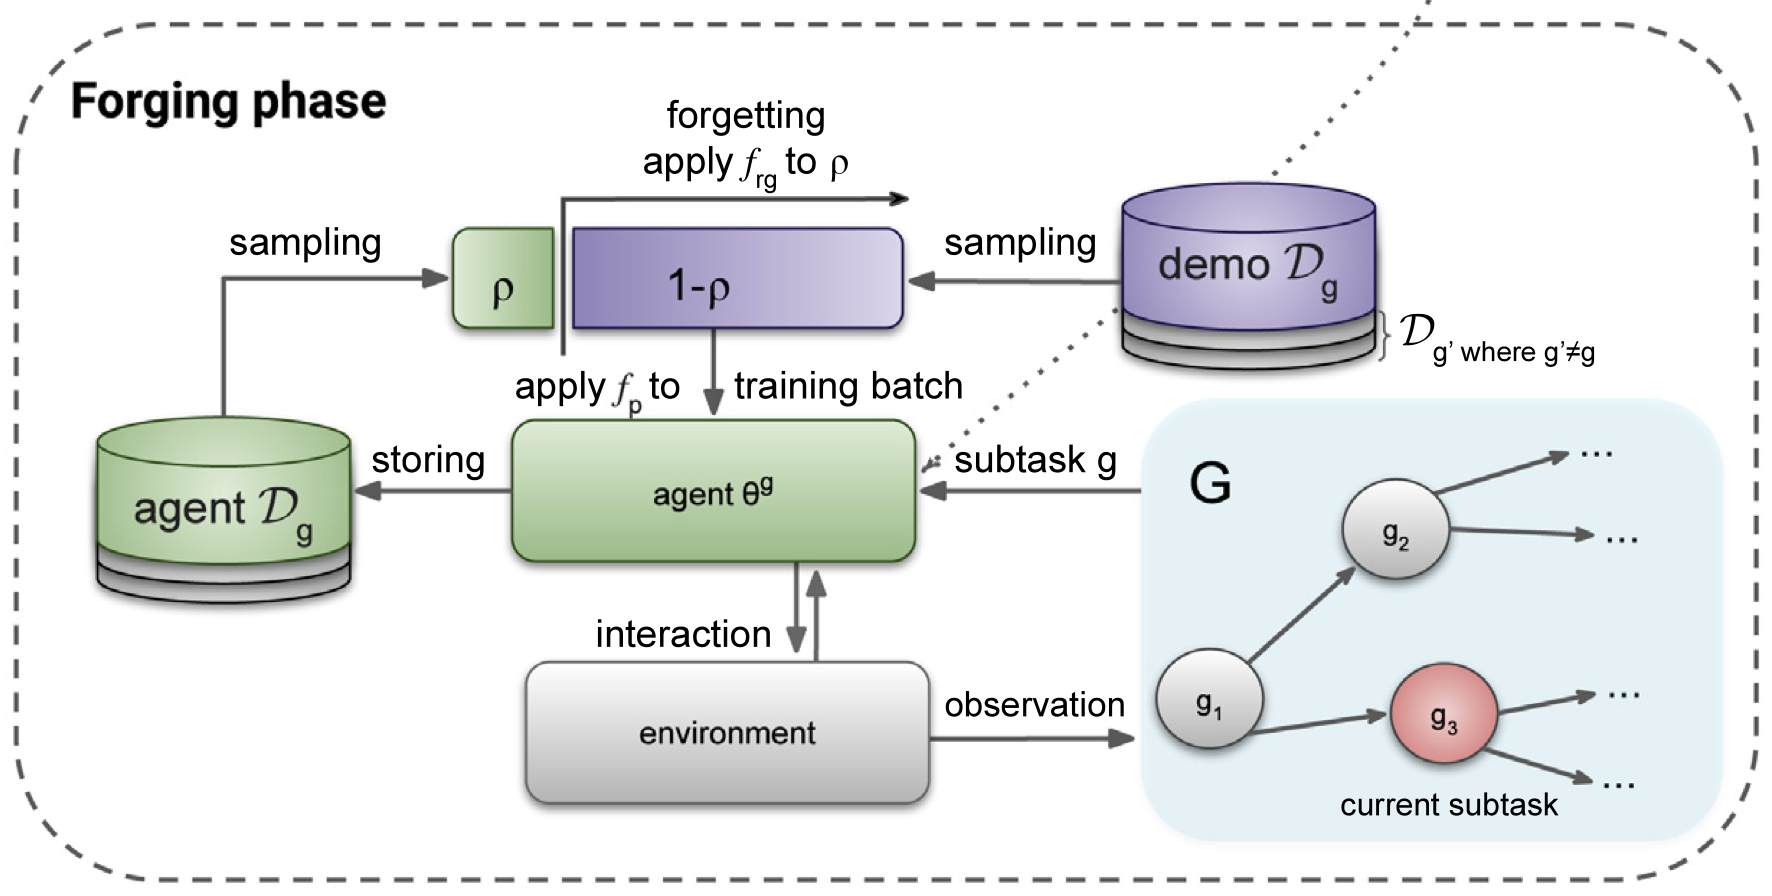
\includegraphics[width=0.6\textwidth]{background/fyp16-forger-arch.png}
  \caption{ForgER with dynamic sampling between demonstration and own experience buffers.}
\label{fig:fyp16-forger-arch}
\end{figure}

ForgER makes use of hierarchical experience replay techniques paired with managed forgetting to address the choice of retention and discarding of experiences. 
The proposed algorithm allows for the extraction of subgoals from expert data based on different sections of a complex trajectory. 
Then, for each identified subgoal, a replay buffer is populated with goal-specific demonstration data. 
Finally, a Forgetful Experience Replay algorithm, which accumulates the agent's own experiences of the subtask while progressively phasing out demonstration data.
This Forgetful Experience Replay is what we will focus on here.

The algorithm is motivated by the recognition of the suboptimality of expert demonstrations and the potential discrepancy between the state space of the expert and the agent.
This discrepancy frequently arises due to simplifications of the environment for the agent, such as discretising a continuous state space.
The paper explores three approaches for sampling from the replay buffers.
The first involves maintaining all experiences in a single buffer and sampling uniformly.
The second strategy entails storing data in two separate buffers and sampling evenly between demonstration data and the agent's own experiences.
The third, and the method proposed by this paper, dynamically adjusts the sampling ratio between the two buffers, as shown in Figure~\ref{fig:fyp16-forger-arch}.

In this context, forgetting is the process of gradually reducing the dependency on demonstration data as the agent progressively learns from its own experiences.
This can be implemented linearly as: 
\[f_{rg}(k) = \min(1, k/d)\]
This effectively manages the balance between leveraging demonstration data and incorporating the agent's personal experiences.
This presents an interesting approach to utilising demonstration data, ensuring a balance between the integration of expert knowledge with the agent's autonomously gained insights. \\\\

\section{Inverse Reinforcement Learning}
% FYP7 - "An Application of Reinformcent Learning to Aerobatic Helicopter Flight (P. Abel 2007)" - Demonstration
One of the earliest applications of Reinforcement Learning (RL) in a real-world 3 dimensional space was in Aerobatic Helicopter Flight~\cite{abbeelRLAerobaticFlight}.
Inverse Reinforcement Learning (IRL) was employed to learn a helicopter model and its associated reward function from human demonstrations.
This led to the first successful autonomous completion of four complex manoeuvres.
This approach was motivated by the high amount of exploratory searching required in conventional Reinforcement Learning, which would lead to unsafe conditions and crashes.
Instead, Apprenticeship Learning was employed, allowing the system to create a model from demonstration flight data for each manoeuvre.
This model was then tested in simulation before finally being tried out on a physical helicopter.
The reward function consisted of 24 components, and the balance between them was defined via an IRL algorithm.
However, they found that strictly following the reward weights generated by this algorithm often led to unsafe conditions for the helicopter.
So, the reward weights were iteratively hand-chosen from a mixture of the algorithm suggestions and the authors' intuition. 
To address the risk of an unstable policy that was prone to fluctuating between extreme values, a term was added to the reward function, penalising change in inputs over successive time steps.

In the case of two manoeuvres, a single iteration of the process involving just 5 minutes of demonstration flight data proved sufficient to generate an accurate safe manoeuvre.
For the remaining two manoeuvres, this process was repeated twice using further flight data to achieve a good result.
This study demonstrates that it is possible to effectively utilise demonstration data to massively speed up the training of a reinforcement agent.
This particular work led to further exploration in the field of using demonstration data and IRL when trying to achieve a solution in areas where reward functions were difficult to manually define.

However, a notable limitation of this approach is its reliance on expert-generated demonstration data.
The demonstration data is presumed to represent the optimal solution, an assumption that is unlikely to hold in the vast majority of applications.
The agent's performance is inherently limited by the expertise of the demonstrator.
Since the reward function is established from the demonstration data, there lacks a mechanism to reward or even acknowledge improvements beyond the demonstrated capabilities.
This presents a challenge in scenarios where expert data is not necessarily possible or where surpassing the skill of a human pilot is required. \\\\


\section{Reinforcement Learning from Demonstrations}

% - FYP9 - DeepQ Learning from Demonstration

More recent advancements in integrating demonstration data in training have utilised deep learning techniques to achieve significant success~\cite{deepQLearningFromDemo}.
An algorithm, Deep Q-learning from Demonstrations (DQfD) was developed that makes use of a very small set of demonstration data to speed up the training time.
The performance of DQfD was evaluated using Atari Games, a popular benchmark in RL, DQfD outperformed its counterparts during the first million stages on 41 of 42 games and achieved state-of-the-art scores in 11 games.
This research was motivated by the unavailability of an accurate simulation environment.
DQfD incorporates a primary phase where the agent samples purely from a set of demonstrations.
Multiple loss functions were employed, including supervised loss which was essential for the pre-training phase.
By its nature, demonstration data covers a very narrow margin of the state space, often excluding potentially hazardous actions.
However, simply using the demonstration data as part of an experience replay buffer is not sufficient as the agent will not adequately learn that these non-provided actions are more likely to be dangerous.
Without this supervised loss, the agent might favour these unseen areas of the state space which are likely to contain dangerous actions.
L2 regularisation loss was used upon the weights and biases in the network to ensure that the agent doesn't overfit considering the very small number of demonstration examples.
By incorporating these elements, DQfD accelerates the training process.

Once pre-training is complete, the system begins interacting with the actual environment, collecting additional data in a manner similar to standard DQN learning.
These additional experiences are collected in a replay buffer along with the original demonstration examples.
The demonstrated data is always kept in the buffer and not overridden, additionally, it is sampled at a higher frequency than the agent-collected data.
This effectively treats the demonstrated data as a special type of collected data.
This provides a balance between the imitation and further exploration of the state space to produce ``superhuman'' results.
The DQfD agent has a strong resilience to suboptimal demonstrations or outliers.
The agent outperformed the worst demonstration provided in 29 out of 42 games.
In 14 of the 42 games, the agent was able to surpass the performance of the best demonstration provided, further proving the possibility for improvement beyond the provided examples; achieveing state-of-the-art in 11 games.

This research shows the potential ability to overcome some of the difficulties encountered in the drone perching environment where the dynamics of the environment are complex to simulate.
This study demonstrates that utilising demonstration data can be a valuable way to address the safety aspects encountered when using real-world environments.
This is achieved with a relatively small amount of demonstration data from several minutes of gameplay per game.
However, it is unknown whether just demonstration data alone would provide enough safety for drone trajectories.
Additionally increasing the performance from the demonstration data still requires a high number of training episodes.
Although this is certainly an improvement, it would likely still take a very large amount of training time to successfully improve which is key to becoming better than the given demonstrations and allowing a drone to develop good trajectories from non-expert demonstrations.

This research only covers domains with discrete action spaces, in the drone perching environment, we have the ability to perform actions across a continuous action space.
This is likely to be more computationally expensive which is another challenge that will need to be overcome.
One of the major differences is the reward associated.
In the Atari games environment, the reward is tied directly to the score achieved by the agent, this makes evaluating performance clear.
However, in the drone perching environment this is more challenging.
It is not immediately clear how to balance rewards between actually achieving the perching action, with safety to prevent crashes and speed and energy efficiency.
This makes evaluating the performance less clear.
This makes the task of defining a reward function more complex and less straightforward to define. \\\\

%     - FYP14 - Learning from Imperfect Demonstrations
In the area of learning from demonstrations, it is usually assumed that the demonstration data provided is expert behaviour.
Although there is the possibility of improving from these demonstrations, the improvements are often minor and imperfect demonstrations can have a large performance impact.
However, in real-world scenarios, the demonstrations provided are often sub-optimal, this is critical when there is a requirement to improve beyond the demonstration data.
To address these challenges, the Normalised Actor-Critic (NAC) method has been proposed, showing robustness against poor or even detrimental demonstrations~\cite{fyp14-rl-imperfect-demos}.

Demonstrations are typically a highly biased sample of the environment.
For example, it is unlikely that a demonstration dataset includes a drone crash scenario.
Although alternative algorithms can understand that demonstration data is generally good, they often have no ability to understand that alternative actions are potentially worse.
This lack of negative based demonstrations, especially in off-policy learning, can lead to unintended consequences.
The NAC approach introduced a soft policy gradient that reduced the Q-values of actions not present in demonstrations.
This differs from the standard soft Q-learning gradient, defined as $ \Delta_{\theta} Q_{\theta}(s, a)(Q_{\theta}(s, a) - \hat{Q}_{\theta}(s, a)) $.
The normalised version includes an additional term, $\Delta_{\theta} V_Q(s)$, preventing the inflation of Q-values for actions that are unseen:
\[ (\Delta_{\theta} Q_{\theta}(s, a) - \Delta_{\theta} V_Q(s))(Q_{\theta}(s, a) - \hat{Q}_{\theta}(s, a))\]

\todo{seperate this maths}

The full algorithm has been reproduced here in Algorithm.~\ref{alg:nac-imperfect-demos}.

\begin{algorithm}
\label{alg:nac-imperfect-demos}
\caption{Normalised Actor-Critic for Learning from Demonstration~\cite{fyp14-rl-imperfect-demos}}
\begin{algorithmic}[1] % The number tells where the line numbering should start
\State Initialize parameters $\theta$ for the rapid Q network, $\theta'$ for the target Q network
\State Initialize $D$: demonstrations collected by humans or a trained policy network
\State Initialize $T$: target network update frequency
\State Initialize $M$: replay buffer
\State Initialize $k$: number of steps to train on the demonstrations

\For {$t = 1, 2, \dots$} % The range of t
    \If {$t \leq k$}
        \State Sample a mini-batch of transitions from $D$
    \Else
        \State Start from $s$, sample $a$ from $\pi$, execute $a$, observe $(s',r)$
        \State Store $(s, a, r, s')$ in $M$
        \State Sample a mini-batch of transitions from $M$
    \EndIf
    \State Update $\theta$ with gradient: $\nabla_\theta J_{PG} + \nabla_\theta J_V$
    \If {$t \mod T = 0$} % Condition for updating the target network
        \State $\theta' \gets \theta$
    \EndIf
\EndFor
\end{algorithmic}
\end{algorithm}

This algorithm was compared with the Deep Q-learning from demonstrations algorithm~\cite{deepQLearningFromDemo} in a Minecraft style environment, and two driving games; Torcs and GTA.
The NAC algorithm has shown remarkable performance.
Overall NAC performed marginally better than DQfD in the Torcs game but significantly stronger in the GTA game especially when the agent is allowed to interact with the real environment after demonstrations.
The true advantage of NAC becomes evident when leveraging imperfect demonstrations.
With datasets containing 30\%, 50\%, and 80\% imperfect data, NAC's performance only marginally decreases, whereas the performance of DQfD drops to approximately 40\% of the original under higher imperfect demonstration percentages.
NAC's ability to learn beneficial behaviours while avoiding suboptimal ones is extremely effective.

NAC is resilient to imperfect demonstrations, this is particularly beneficial in real-world scneraios where providing good demonstrations is difficult.
It enables the collection of demonstrations, followed by continuous, safe training in real-world conditions. \\\\


% FYP17 - Mapless navigation for UAVs via Reinforcement Learning
\todo{swap around this and the previous one}
In other areas of Reinforcement Learning variants of the Soft Actor Critic Algorithm have performed well.
Motivated by the lack of success from DQfD in complex environments, an algorithm, Soft Actor Critic from Demonstrations (SACfD) was proposed~\cite{SACfDMaplessNavigation}.
This aimed to combine the strong success of SAC algorithms in complex environments.
The aim of this task was to navigate a drone towards a destination while avoiding obstacles in a simulation environment.

\begin{figure}[htbp]
  \centering
  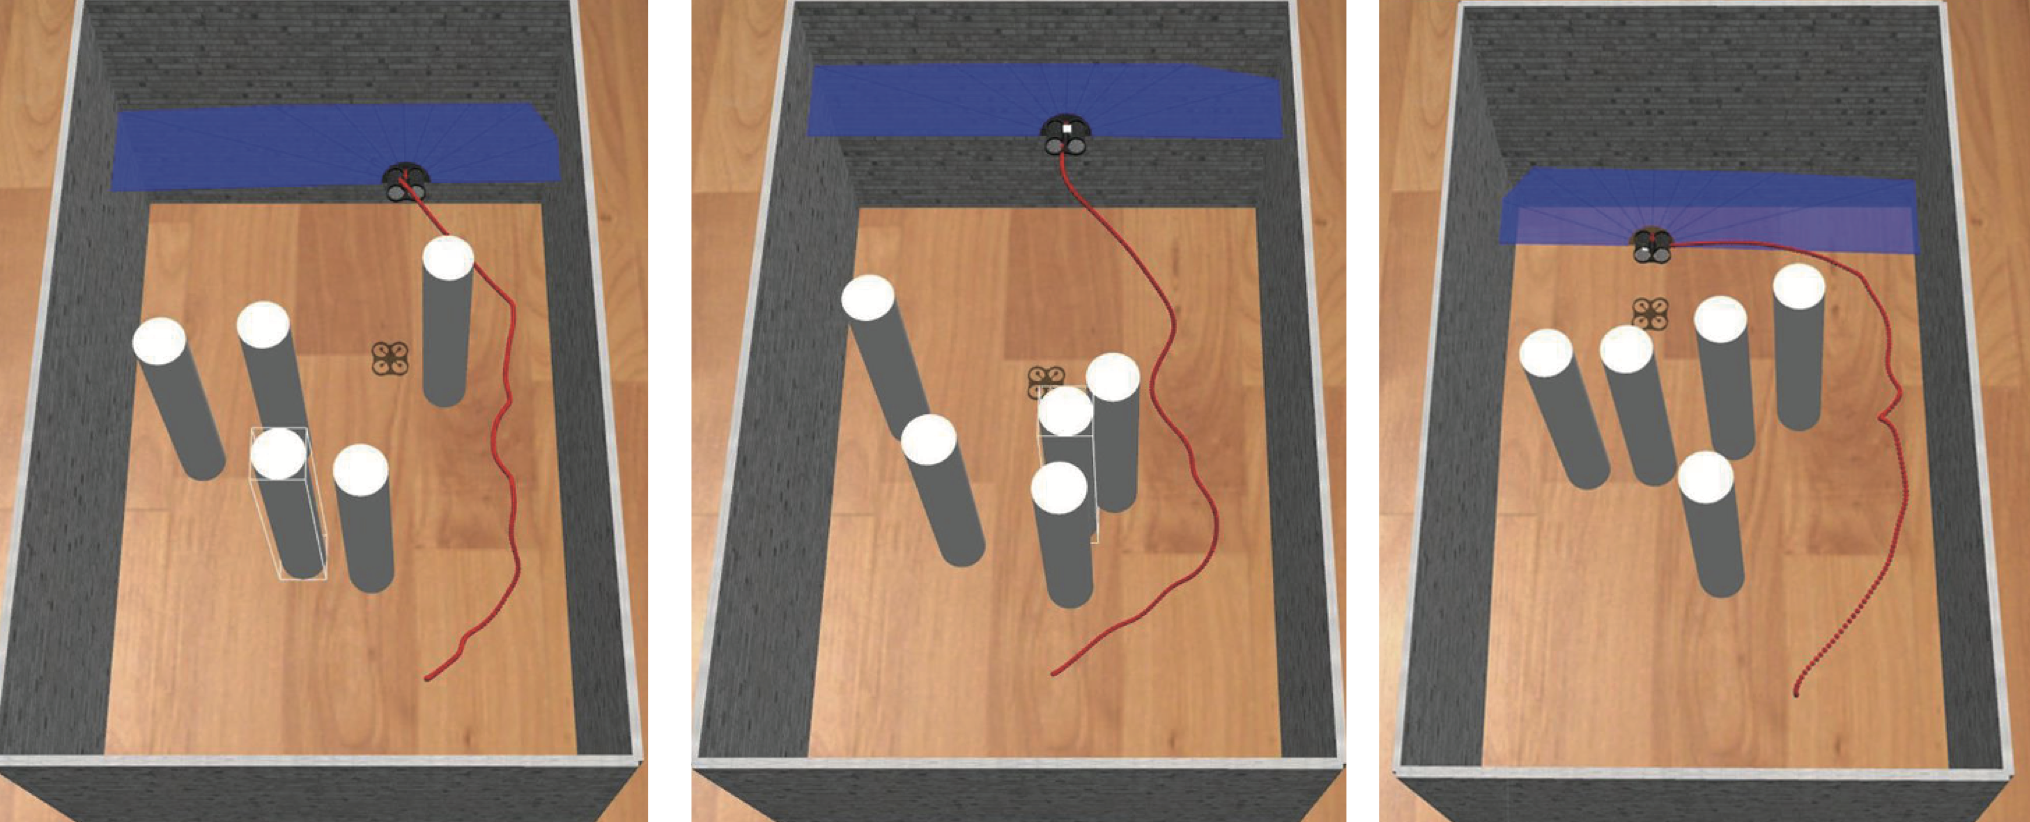
\includegraphics[width=\textwidth]{background/fyp17-sacfd.png}
  \caption{Mapless navigation environment for Soft Actor Critic from Demonstrations}
\label{fig:fyp17-sacfd}
\end{figure}

The reward used 3 cases as shown in Equation.~\ref*{eq:fyp17-sacfd-reward}. 
The final case effectively shows a heuristic was used to increase rewards closer to encourage the agent to rate positions closer to the destination as higher.
\todo{do this for all of the maths}
\begin{equation}
  r(s_{t}, a_{t}) =
  \begin{cases} 
    r_{arrive} & |x_{t} - g_{t}| < \delta \\
    r_{obstacle} & l_{t} < \epsilon \\
    1-0.1 |x_{t} - g_{t}| & \text{otherwise}
  \end{cases}
  \label{eq:fyp17-sacfd-reward}
\end{equation}

One of the most interesting parts of this particular paper was its effective use of coordinate frames.
The aim for the agent was to learn to aviod obstacles.
Rather than being provided with a view on the map or locations of the obstacles, observations were provided around the drone, which effectively gave distances to obstacles in each direction around the drone.
This effectively measures everything from a drone coordinate frame.
Within the particular drone perching task, the choice of coordinate frames is more complex, since there are multiple relations between objects that are important to account for.
There is the drone itself, the perching branch and also the tether.
In particular since the dynamics between the tether and the drone are complex to model in simulation, this is an area where demonstration could be a very useful application.
\todo{diagram showing lazer view}
An interesting observation in this paper is that many reinforcement learning algorithms are trained on a single map.
One of the major aims here was in generalisation and the understanding of measurements for any map rather than "memorizing" a particular map.
Therefore in this environment, the positions of the obstacles and destination were randomly assigned in each episode to ensure that generalisation from observations occurred.
One area of note in this particular example is the trajectories that this algorithm generates are largely not smooth and could prove complex and non-efficient to actually fly in a real environment.

\todo{improve diagram showing the environment}


\section{Transfer Learning}
%     - FYP10 - Soft Actor-Critic with Inhibitory Networks for Retraining UAV Controllers Faster
Transfer Learning is a growing field in Reinforcement Learning.
This approach addresses a key limitation of traditional RL, where each new task typically requires restarting the learning process from scratch.
A process that can be quite time-consuming. 
Transfer learning facilitates the reuse of skills acquired from one task for use in another task, thereby significantly accelerating the training process.

In the specific context of UAVs, real-world datasets are often limited or time-consuming to collect.
Transfer learning can be employed to accelerate training time.
Much of the current work, involves training an RL agent within a simulated environment, where interactions are both less resource-intensive and also considerably faster. 
The skills learnt in this simulated setting are then transferred to agents designated for real-world tasks.
Expanding on this, there is often a need for learning multiple distinct but related tasks.
Traditional approaches necessitate separate training for each new task, transfer learning allows for the use of skills learned from an initial task to later subsequent ones, accelerating the training process for this second task.

The conventional Soft Actor Critic (SAC) employs a single parameter responsible for balancing exploration against learned skills.
This is not particularly suitable to be used for learning new skills since it often results in catastrophic forgetting of previously learned skills~\cite{fyp10-initial-transfer-learning}.

To mitigate this issue, the Soft Actor Critic with Inhibitory Networks (SAC-I) has been proposed~\cite{fyp10-sac-Inhibitory}.
SAC-I introduces inhibitory control into the SAC framework, inhibitory control is defined as the capacity to stop ongoing or planned processes.
This model uses a dual-critic system, each tailored to a specific task.
When learning a new related task, the model does not start from scratch.
It introduces a new set of Q-values specific to the new task, maintaining both sets of networks within the same system. 
A critical component of SAC-I is the introduction of an inhibition rule, which controls which network is utilised based on environmental conditions.
This not only keeps the knowledge from previous tasks but also ensures a more efficient training process in learning new tasks, addressing the issue of catastrophic forgetting and enhancing the overall efficacy of the training process.

\begin{figure}[htbp]
  \centering
  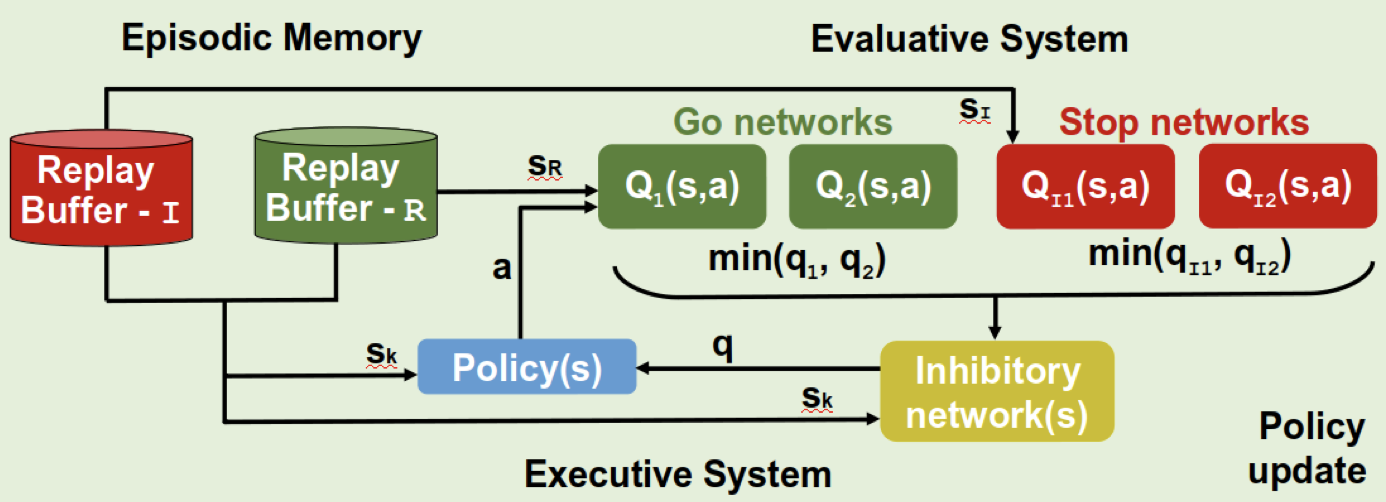
\includegraphics[width=\textwidth]{background/fyp-10-sac-inhibitors.png}
  \caption{Soft Actor Critic with Inhibitory Networks Architecture Design}
\label{fig:fyp17-sacfd}
\end{figure}

During the training phase, initially, a primary network is trained on an original task.
Subsequently, a secondary network is introduced, inheriting the initial weights from the primary network.
The training process then continues for the second task and is carried out on both networks, guided by an inhibitory rule that classifies between the scenarios.

This dual-network system was validated in an obstacle avoidance scenario.
Initially, a UAV was trained to navigate to its destination point using a traditional Soft Actor Critic (SAC) network. 
Following this, the Soft Actor Critic with Inhibitory Networks (SAC-I) was introduced. 
Initially, both networks in the SAC-I framework copied their weights from the SAC network that had been previously trained. 
Finally, the UAV retrained, with the secondary network focusing specifically on obstacle avoidance and dynamically switching between networks when proximity to an obstacle was detected. 
This structured approach significantly increased the speed of the training process.


Effectively this methodology gives the agent the capacity to deconstruct complex tasks in a manner akin to Hierarchical Reinforcement Learning (HRL). 
Applying this directly to the drone perching example, this could be used to model different sections of the task.
For instance, the initial phase could concentrate on mastering the wrapping of the tether, followed by training on the subsequent phase of drone disarmament. 
The primary advantage of this system is the consolidation of task-specific networks into a unified system.

However, a critical limitation of this approach is the need for manually defining the distinct tasks within the overall objective. 
Furthermore, the degree of overlap between different task phases remains unclear. 
For instance, while the flight dynamics in separate phases may exhibit similarities, however given the different goals and objectives of the different phases, it is unknown how well this would perform in practice. \\\\


%     - FYP-15 - Demonstration Guided Reinforcement Learning with Learned Skills
Traditional Demonstration Guided RL as previously discussed, is able to combine both a set of demonstrations with reward feedback to learn complex behaviours.
Traditional approaches treat every new task as a completely different learning problem which incurs the cost of training time.
In real-world examples such as drone perching, demonstrations and indeed exploration is extremely expensive.
One way to reduce this cost is by reusing skills between multiple different tasks.
Motivated by the fact that most tasks are comprised of many reusable skills, Skill-based Learning with Demonstrations (SkiLD) has been proposed~\cite{fyp15-demo-guided-rl-with-skills}.

SkiLD aims to improve the efficiency of traditional techniques using previous experiences from different tasks.
In SkiLD this takes the form of a task-agnostic dataset, this is experiences that are not necessarily trained on the particular task but can come from any related task.
This dataset $D = \{s_t, a_t, \dots\}$ consists of agent behaviours from any related task.
A secondary dataset $D_{demo} = \{s_{t}^{d}, a_{t}^{d}, \dots\}$ are task-specific demonstrations, these are demonstrations from the current task that the agent is attempting to solve.
From here a set of skills are extracted from the task-agnostic dataset as shown in Figure~\ref{fig:fyp15-skild}.

\begin{figure}[htbp]
  \centering
  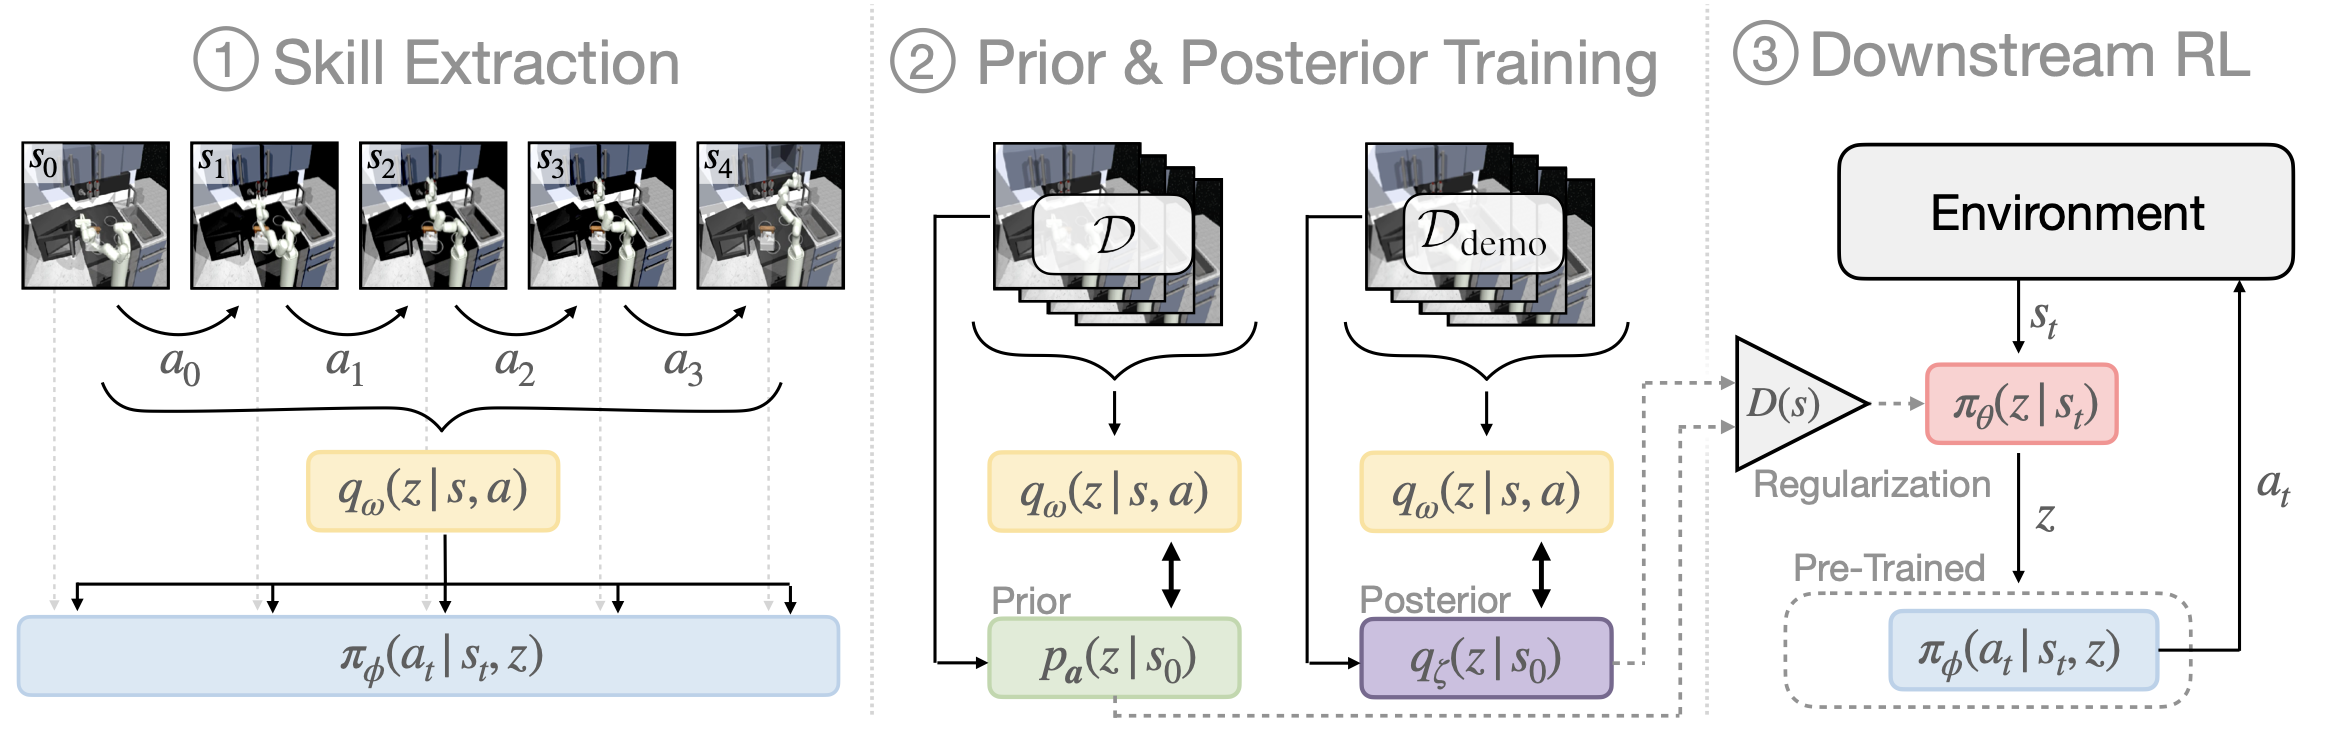
\includegraphics[width=\textwidth]{background/fyp15-skild-architecture.png}
  \caption{Skill-based Learning with Demonstrations Architecture}
\label{fig:fyp15-skild}
\end{figure}

Target demonstrations are used to learn a task-specific skills posterior.
From here the algorithm aims to utilise the skills posterior when closely aligned to the demonstrations, and utilise the skills prior and also encourage the policy to match states within the demonstration support.

\begin{figure}[htbp]
  \centering
  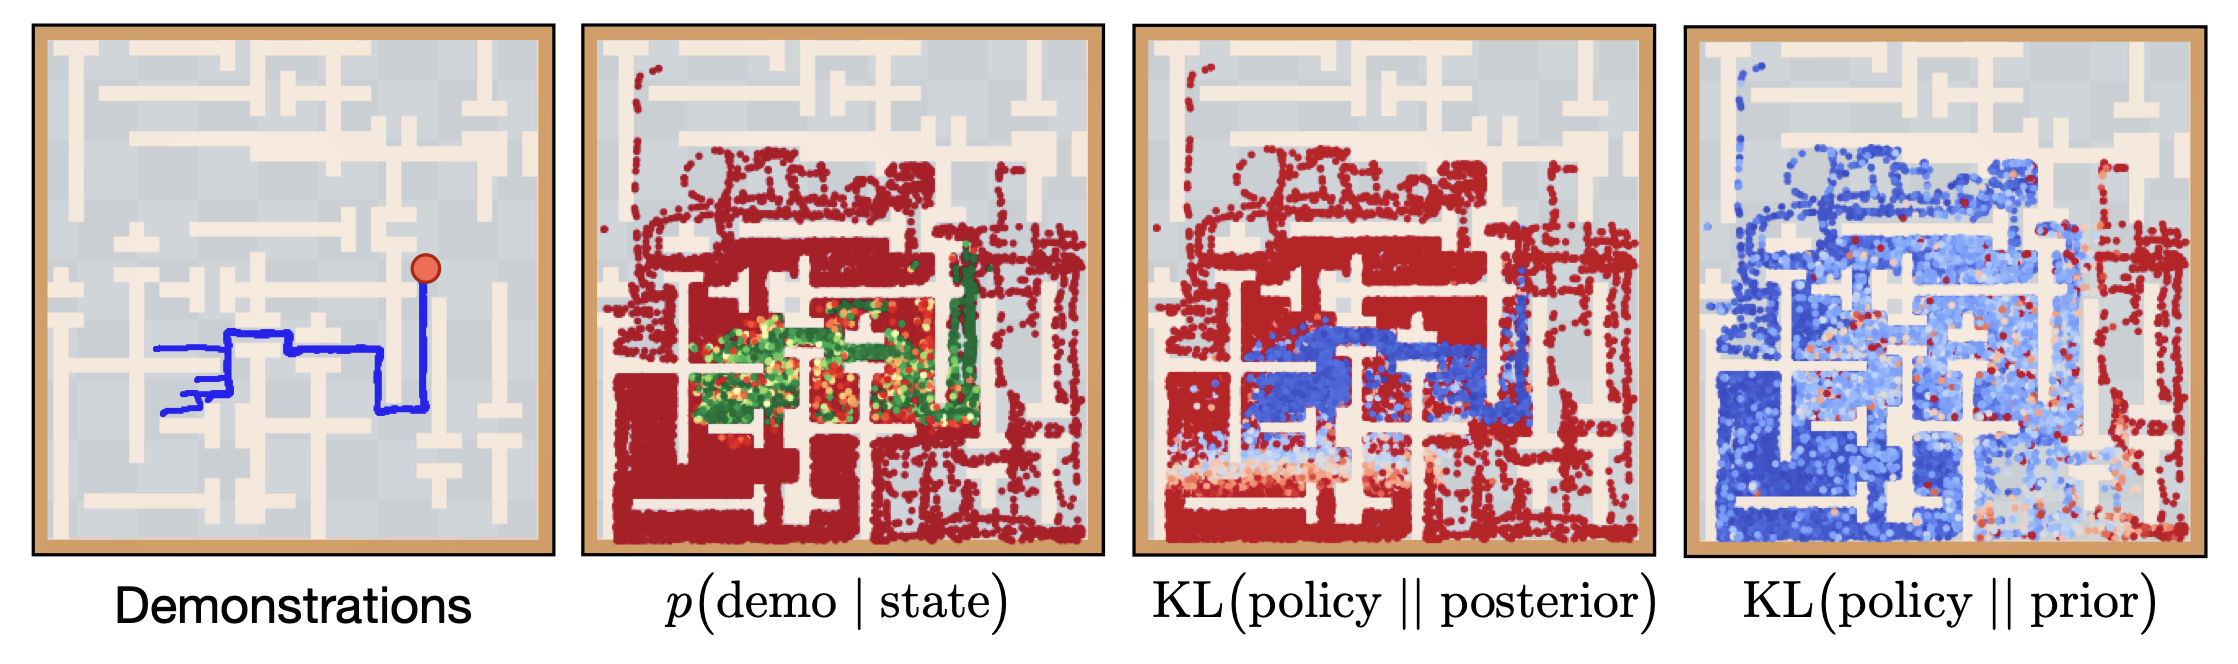
\includegraphics[width=\textwidth]{background/fyp15-maze-diagram.png}
  \caption{Visualisation of Maze Environment}
\label{fig:fyp15-maze}
\end{figure}

This system was evaluated in three different environments, one of which being a maze navigation environment.
Figure~\ref{fig:fyp15-maze} shows a visualisation of the maze environment with the skills distributions.
The SkiLD algorithm is able to learn very fast from just 5 task-specific demonstrations, showing faster performance than any comparable algorithm in this environment.

This provides some inspiration in a drone-perching context.
Since there is non-task-specific data for drone flight readily available this could be used in order to speed up the process.
This could further reduce the reliance on the number of demonstrations required.